%%This is a very basic article template.
%%There is just one section and two subsections.
%--------------------------------------------------
\documentclass[letterpaper]{report}  
%--------------------------------------------------
%Packages 
%--------------------------------------------------
\usepackage[english]{babel}
\usepackage{amsmath,amssymb,amsfonts} % Typical maths resource packages
\usepackage[dvips]{graphicx}
\usepackage{color}                    % For creating coloured text and background
\usepackage{fancyhdr}                 % For inclusion of title at the top of the page
\usepackage[left=3cm,right=1.5 cm,top=2cm,bottom=2cm,bindingoffset=0cm]{geometry}
\usepackage[explicit]{titlesec}
\usepackage{setspace}
\usepackage{pdfpages}
\usepackage{cite} 
\usepackage{float} 
\usepackage{newclude}
\usepackage{bookmark}
\usepackage{listings}
\usepackage{tikz}
\usepackage{type1cm}
\usepackage{textcomp}
\usepackage{hyperref}                  % For creating hyperlinks in cross
\usetikzlibrary{fit}
   
\definecolor{mygreen}{RGB}{28,172,0} % color values Red, Green, Blue
\definecolor{mylilas}{RGB}{170,55,241}
\definecolor{grey}{rgb}{0.97,0.97,0.97}
\newcommand*\chapterlabel{}
\makeatletter
\def\@makechapterhead#1{%
  \vspace*{10\p@}%
  {\parindent \z@ \centering \reset@font
        \par\nobreak
        \vspace*{2\p@}%
        {\Huge \bfseries \thechapter\quad #1\par\nobreak}
        \par\nobreak
        \vspace*{2\p@}%
    \vskip 40\p@
    %\vskip 100\p@
  }}
\def\@makeschapterhead#1{%
  \vspace*{10\p@}%
  {\parindent \z@ \centering \reset@font
        \par\nobreak
        \vspace*{2\p@}%
        {\Huge \bfseries #1\par\nobreak}
        \par\nobreak
        \vspace*{2\p@}%
    \vskip 100\p@
    %\vskip 100\p@
  }}
\makeatother

\newcounter{N}
\setlength{\parindent}{0ex}
\setlength{\parskip}{1em}

\lstset{language=Matlab,
basicstyle=\footnotesize\ttfamily,
basewidth=0.5em,
morekeywords={matlab2tikz},
keywordstyle=\color{blue},%
morekeywords=[2]{1}, keywordstyle=[2]{\color{black}},
identifierstyle=\color{black},%
stringstyle=\color{mylilas},
commentstyle=\color{mygreen},%
numbers=none,
numberstyle=\tiny\color{black},
stepnumber=2, 
numbersep=10pt,
tabsize=4,
aboveskip=3mm,
belowskip=3mm,
backgroundcolor=\color{grey},
frame=none,
showspaces=false,
showstringspaces=false,
breaklines=true}

\begin{document}
\begin{titlepage}
\begin{center}
\vspace{5cm}
{\bfseries\href{https://www.portfolioeffect.com}{www.portfolioeffect.com} \\
High Frequency Portfolio Analytics\\}
\vspace{8cm}
{\huge User Manual \\}
\vspace{0.3cm}
{\Huge\bfseries PortfolioEffectEstim \\ MATLAB Toolbox \\}
\vspace{0.4cm}
{\Large High Frequency Price Estimators \& Models \\}
% ----------------------------------------------------------------
\vspace{1.5cm}
{Andrey Kostin \\ andrey.kostin@portfolioeffect.com} \\[14pt]
 % ----------------------------------------------------------------
\vfill
\emph{{Released Under BSD License\\ by Snowfall Systems,
Inc.}}\\[2cm]
{August 20, 2015}
\end{center}
\end{titlepage}

\bookmarksetup{startatroot}
\cleardoublepage
\phantomsection
\addcontentsline{toc}{chapter}{Contents}
\bibliographystyle{amsplain}%}
\renewcommand{\bibname}{Contents}
\tableofcontents 
%\VignetteIndexEntry{PorfolioEffectEstim package}

\chapter{Toolbox Installation}
PortfolioEffect Estimators Toolbox for MATLAB is provided as a zip archive for
all types of operating systems and as a self-install executable file for Windows. 

\section{Zip Archive (All OS)}
Download zip archive with a toolbox from
PortfolioEfect
\href{https://www.portfolioeffect.com/docs/platform/quant/downloads}{downloads}
or MATLAB Central
\href{http://www.mathworks.com/matlabcentral/fileexchange}{File Exchange}.

Once downloaded, unpack archive into the folder and add
PortfolioEffectEstim folder to MATLAB's path using 'Set Path' menu. Then call
any method of the package in MATLAB editor to continue with the set-up:
\begin{lstlisting}
+++++++++++++++++++++++++++++++++++++++++++++++++
Welcome to PortfolioEffect Estimators Toolbox.

Setup will download required binary files (~5mb).
Please, wait...
SUCCESS. File downloaded to: 
/home/appadmin/.matlab/R2015a/portfolioeffect-quant-client-1.0-allinone.jar
Updating java class path file...
SUCCESS. Java class path updated.

Setup complete! Restart Matlab session now.
+++++++++++++++++++++++++++++++++++++++++++++++++
\end{lstlisting}

Restart MATLAB to complete installation.

\section{Install Wizard (Windows)}
Download self-installeer executable for Windows from PortfolioEfect
\href{https://www.portfolioeffect.com/docs/platform/quant/downloads}{downloads}.
Follow the installation instructions. Once the wizard completes, add the
PortfolioEffectEstim folder to MATLAB's path using 'Set Path' menu. 
The PortfolioEffect Estimators Toolbox is now fully configured.

\chapter{Account Credentials}
All computations are performed on PortfolioEffect cloud servers.
To obtain a free non-professional account, you need to follow a quick sign-up
process on our website:
\href{https://www.portfolioeffect.com/registration}{www.portfolioeffect.com/registration}.\par
Please use a valid sign-up address - it will be used to email your
account activation link.

\section{Locate API Credentials} 
Log in to you account and locate your API credentials on the main page

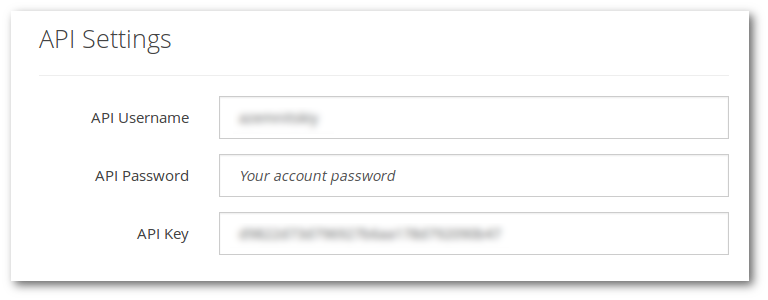
\includegraphics[width=5in,natwidth=768,natheight=300]{img/api-settings.png}
 
\section{Set API Credentials in MATLAB} 
Run the following commands to set your account API credentials for the
PortfolioEffect Estimators Toolbox for MATLAB.
You will need to do it only once as your credentials are stored between sessions
on your local machine to speed up future logons. \par You would need to repeat
this procedure if you change your account password or install PortfolioEffect
toolbox on another computer.
\begin{lstlisting}
util_setCredentials('API Username', 'API Password', 'API Key');
\end{lstlisting}
You are now ready to call PortfolioEffect methods.

\chapter{Estimator Construction}
\section{User Data}
Users may supply their own historical datasets for asset entries. 
This external data could be one a OHLC bar column element (e.g. 1-second close prices) or a vector of actual transaction prices that contains non-equidistant data points. 
% You might want to pre-pend at least N =(4 x windowLength) data points to the
% beginning of the interval of interest which would be used for initial calibration of portfolio metrics.
\subsection{Create Estimator}
Method
\href{https://www.portfolioeffect.com/docs/platform/quant/functions/general-functions/estimator-create}{estimator\_create()}.
takes a vector of asset prices in the format (UTC timestamp, price) with UTC
timestamp expressed in milliseconds from 1970-01-01 00:00:00 EST.
\begin{lstlisting}
      Time          Value
   1.4123e+12       568.45
   1.4123e+12       567.46
   1.4123e+12       567.86
   1.4123e+12       567.53
   1.4123e+12          568
\end{lstlisting}
If asset symbol is specified, it is silently ignored.
\begin{lstlisting}
data_spy=importdata('data_spy.mat'); 

% Create estimator
estimator=estimator_create('priceData',data_spy);
\end{lstlisting}

\section{Server Data}
At PortfolioEffect we are capturing and storing 1-second intraday bar history for a 
\href{https://www.portfolioeffect.com/docs/symbology}{all NASDAQ traded equites}.
This server-side dataset spans from January 2013 to the latest trading time minus five minutes. 
It could be used to construct asset estimators and compute intraday estimator metrics.
\subsection {Create Estimator}
Method
\href{https://www.portfolioeffect.com/docs/platform/quant/functions/general-functions/estimator-create}{estimator\_create()}
creates new asset estimator or overwrites an existing estimator object with the
same name. \par
When using server-side data, it only requires a time interval that would be treated.
\par
Interval boundaries are passed in the following format:
\begin{itemize} 
  \item 'yyyy-MM-dd HH:MM:SS' (e.g. '2014-10-01 09:30:00')
  \item 'yyyy-MM-dd' (e.g. '2014-10-01')
  \item 't-N' (e.g. 't-5' is latest trading time minus 5 days)
  \item UTC timestamp in milliseconds (mills from '1970-01-01 00:00:00') in EST
  time zone
\end{itemize}
\begin{lstlisting}
% Timestamp in "yyyy-MM-dd HH:MM:SS" format
estimator=estimator_create('asset','AAPL','fromTime','2014-09-01 09:00:00','toTime','2014-09-14 16:00:00');

% Timestamp in "yyyy-MM-dd" format
estimator=estimator_create('asset','AAPL','fromTime','2014-09-01','toTime','2014-09-14');

% Timestamp in "t-N" format
estimator=estimator_create('asset','AAPL', 'fromTime','t-5','toTime','t');
\end{lstlisting}

\subsection {Get Symbols List}
Once estimator is created, 
\href{https://www.portfolioeffect.com/docs/platform/quant/functions/general-functions/estimator-available-symbols}{estimator\_availableSymbols()} 
method could be called to receive the list of all available symbols for asset creation. 
Each symbol is accompanied by a full company/instrument description and listing exchange name.

\begin{lstlisting}
estimator_availableSymbols(estimator)

      id      description                                                 exchange  
 [1,] "BBC"   "BioShares Biotechnology Clinical Trials Fund"              "NASDAQ"  
 [2,] "SCS"   "Steelcase Inc. Common Stock"                               "NYSE"    
 [3,] "BBD"   "Banco Bradesco Sa American Depositary Shares"              "NYSE"    
 [4,] "BBG"   "Bill Barrett Corporation Common Stock"                     "NYSE"    
 [5,] "STPP"  "Barclays PLC - iPath US Treasury Steepener ETN"            "NASDAQ"  
 [6,] "BBF"   "BlackRock Municipal Income Investment Trust"               "NYSE"      
 [8,] "BBH"   "Market Vectors Biotech ETF"                                "NYSEARCA"
 [9,] "SCON"  "Superconductor Technologies Inc. - Common Stock"           "NASDAQ"  
[10,] "SCX"   "L.S. Starrett Company (The) Common Stock"                  "NYSE"    
[11,] "BBK"   "Blackrock Municipal Bond Trust"                            "NYSE"  
\end{lstlisting}

\chapter{Estimator Settings}

These settings regulate how estimator metrics are computed, returned and stored.
\subsection{Results Sampling Interval}
Interval to be used for sampling computed results before returning them to the caller. 
Available interval values are: 
\begin{itemize} 
  \item 'Xs' - seconds
  \item 'Xm' - minutes
  \item 'Xh' - hours
  \item 'Xd' - trading days (6.5 hours in a trading day)
  \item 'Xw' - weeks (5 trading days in 1 week)
  \item 'Xmo' - month (21 trading day in 1 month)
  \item 'Xy' - years (256 trading days in 1 year)
  \item 'none' - no sampling.
  \item 'last' - only the very last data point is returned  
\end{itemize}
Large sampling interval would produce smaller vector of results and would require less time spent on data transfer. 
Default value of '1s' indicates that data is returned for every second during
trading hours.
\begin{lstlisting}

estimator=estimator_create('asset','AAPL','fromTime','2014-10-01 09:30:00','toTime','2014-10-01 16:00:00');

% sample results every 30 seconds
estimator_settings(estimator, 'resultsSamplingInterval','30s');
variance_30s=variance_tsrv(estimator);

% sample results every 5 minutes
estimator_settings(estimator, 'resultsSamplingInterval','15m');
variance_15m=variance_tsrv(estimator);

util_plot2d(variance_30s,'30s', 'Title','TSRV, resultsSamplingInterval')+...
util_line2d(variance_15m, '15m')
\end{lstlisting}
\subsection{Input Sampling Interval}
Interval to be used as a minimum step for sampling input prices. Available interval values are: 
\begin{itemize} 
  \item 'Xs' - seconds
  \item 'Xm' - minutes
  \item 'Xh' - hours
  \item 'Xd' - trading days (6.5 hours in a trading day)
  \item 'Xw' - weeks (5 trading days in 1 week)
  \item 'Xmo' - month (21 trading day in 1 month)
  \item 'Xy' - years (256 trading days in 1 year)
  \item 'none' - no sampling
\end{itemize}
Default value is 'none', which indicates that no sampling is applied.
\begin{lstlisting}

estimator=estimator_create('asset','AAPL','fromTime','2014-10-01 09:30:00','toTime','2014-10-01 16:00:00');

% sample input prices every 30 seconds
estimator_settings(estimator, 'inputSamplingInterval','30s');
variance_30s=variance_tsrv(estimator);

% sample input prices every 5 min
estimator_settings(estimator, 'inputSamplingInterval','5m');
variance_5m=variance_tsrv(estimator);

util_plot2d(variance_30s,'30s', 'Title','TSRV, inputSamplingInterval')+...
util_line2d(variance_5m, '5m')
\end{lstlisting}

\subsection{Jumps/Outliers Model}
Used to select jump filtering mode when computing return statistics. Available modes are: 
\begin{itemize} 
  \item 'none' - price jumps are not filtered anywhere
  \item 'moments' - price jumps are filtered only when computing return moments
  (i.e. for expected return, variance, skewness, kurtosis and derived
  metrics)
  \item 'all' - price jumps are filtered from computed returns, prices and all
   return metrics.
\end{itemize}
\begin{lstlisting}

estimator=estimator_create('asset','AAPL','fromTime','2014-10-01 09:30:00','toTime','2014-10-02 16:00:00');

% Price jumps detection is enabled for returns and moments
estimator_settings(estimator, 'jumpsModel','all');
variance_all=variance_tsrv(estimator);

% Price jumps detection is disabled
estimator_settings(estimator, 'jumpsModel','none');
variance_none=variance_tsrv(estimator);

util_plot2d(variance_all,'all', 'Title','TSRV, jumpsModel')+...
util_line2d(variance_none, 'none')
\end{lstlisting}


%------------------------------------------------------
\chapter{Price Variance}
%------------------------------------------------------
\section{Integrated Variance}
%------------------------------------------------------
Assume that the logarithmic eqilibrium price of a financial asset is given by the following
diffusion process
\begin{equation}
X_t = \int_0^t \mu(s)ds + \int_0^t \sigma(s)dW(s)
\end{equation}
where

\begin{itemize}
\item $W_t$ is a standart Brownian Motion,
\item the mean process $\mu$ is continuous and of finite variation,
\item $\sigma(t) >0$ denotes the cadlag instantaneous volatility.
\end{itemize}
\noindent The object of interest is the integrated variance $(IV)$, i.e. the
amount of variation at time point $t$ accumulated over a past time interval
$\Delta$ according to ~\cite[Pigorsch et al.]{Pigorsch_Pigorsch_Popov}:
\begin{equation}
IV_t = \int_{t-\Delta}^t \sigma^2(s)ds
\end{equation}
\subsection{Returns}
Suppose there exist $m$ intraday eqilibrium returns, the $i$th intraday return is
then defined as:
\begin{equation}
r_i^{X(m)}= X_{i/m} - X_{(i-1)/m}, \quad i = 1,2,\ldots,m.
\end{equation}
%------------------------------------------------------



%------------------------------------------------------
\section{Realized Variance}
%------------------------------------------------------
\subsection{Assumptions}
The equilibrium price process.
\begin{enumerate}
\item The logarithmic equilibrium price process $p_t^X$
is a continuous stochastic volatility semimartingale. Specifically,
\begin{equation}
p_t^X = \alpha_t + m_t;
\end{equation}
where $\alpha_t$ (with $\alpha_0 =0$) is a predictable drift process of
finite variation and $m_t$ is a continuous local martingale defined as
$\int_0^t\sigma_s dW_s$ with ${W_t: t\geq 0}$ denoting standard Brownian motion.
\item The spot volatility process $\sigma_t$ is cadlag and bounded away from
zero.
\item The process $\int_0^t\sigma_s^4ds$ is bounded almost surely for all $t <
\infty$.
\end{enumerate}
%------------------------------------------------------
\subsection{Estimator}
For discretely observed path $X_{t_i}$, $i = 0,\ldots, n$ of the $X$, the
realized quadratic variation could be estimated consistently using the realized
variance measure, defined as ~\cite[Zu and Boswijk, 2014]{Zu_Boswijk}:
\begin{equation}
RV_t=\sum_{i=1}^n (X_{t_i}-X_{t_{(i-1)}})^2 \stackrel{p}{\to} IV
\end{equation}
However the realized variance estimator for integrated volatility is not consistent when data is
contaminated by market microstrcuture noise. In particular, when we only observe
data with microstructure noise, the realized variance measure will
diverge. When sampling frequency increases, realized variance actually estimates
the sum of infinite many variances of noises.
%------------------------------------------------------
\subsection{Properties}
\begin{itemize}
\item Convergence speed: $m^{1/2}$ ($m$ - number of observation)
\item Unbiased: no
\item Consistent: no
\item Jump Robust: no
\item Allows for time dependent noise: no
\item Allows for for endogenous noise: no
\end{itemize}
\subsection{Usage}
\begin{lstlisting}
variance_rv(estimator)
variance_rvRolling(estimator,wLength)
\end{lstlisting}
 
 
%------------------------------------------------------
\section{Two Series Realized Variance}
%------------------------------------------------------
\subsection{Assumptions}
The microstructure noise.
\begin{enumerate}
\item The microstructure noise, $\epsilon_{t,i}$ , has zero mean and is an
independent and identically distributed random variable.
\item The noise is independent of the price process.
\item  The variance of $\nu_{t,i} = \epsilon_{t,i} - \epsilon_{t,i-1}$ is
$O(1)$.
\end{enumerate}
%------------------------------------------------------
\subsection{Estimator}
Two Scale Realized Variance (TSRV) estimates
integrated volatility consistently. The idea is to use realized variance
type estimators over two time scales to correct the effect of market
microstructure noise. Define as:
\begin{gather}
[Y,Y]^{avg}_t = \frac{1}{K}\sum_{i=K}^n(Y_{t_i} - Y_{t_{(i-K)}})^2\\
[Y,Y]^{all}_t = \sum_{i=1}^n(Y_{t_i} - Y_{t_{(i-1)}})^2\\
\bar{n}=\frac{n-K+1}{K},
\end{gather}
the TSRV estimator is defined as \cite[Zu and Boswijk, 2008]{Zu_Boswijk}:
\begin{equation}
\label{TSRV}
TSRV_t=[Y,Y]^{(avg)}_t - \frac{\bar{n}}{n}[Y,Y]^{(all)}_t \stackrel{p}{\to} IV
\end{equation}
A small sample refinement to the estimator give correction:
\begin{equation}
TSRV_t^{adjust}=\left( 1-\frac{\bar{n}}{n}\right)^{-1} TSRV_t \stackrel{p}{\to} IV.
\end{equation}

\noindent If we have possibly dependent noise we should use an alternative estimator that
is also based on the two time scales idea.

\noindent To pin down the optimal sampling frequency $K$ \cite[Zhang, Mykland, and Ait-Sahalia, 2005]{Zhang_Mykland_Ait-Sahalia}, one can minimize the expected asymptotic variance and to obtain
\begin{equation}
c^* = \left(\frac{16(E\epsilon^2)^2}{TE\eta^2}\right)^{1/3}
\end{equation}

\noindent which can be consistently estimated from data in past time periods
(before time $t_0 = 0$), using $\hat{E\epsilon^2}$ and an estimator of $\eta^2$. $\eta^2$ can be taken to be independent
of $K$ as long as one allocates sampling points to grids regularly. Hence one can choose $c$,
and so also $K$, based on past data.
%------------------------------------------------------
\subsection{Properties}
\begin{itemize}
\item Convergence speed: $m^{1/6}$ ($m$ - number of observation)
\item Unbiased: yes
\item Consistent: yes
\item Jump Robust: no
\item Allows for time dependent noise: no
\item Allows for endogenous noise: no
\end{itemize}
 \subsection{Usage}
\begin{lstlisting}
variance_tsrv(estimator,K)
variance_tsrvRolling(estimator,K,wLength)
\end{lstlisting}
where

\begin{itemize}
\item $K$ is number of subsamples in the slow time series (default: 2)
\end{itemize}

 
%------------------------------------------------------
\section{Multiple Series Realized Variance}
%------------------------------------------------------
\subsection{Assumptions}
Dependent Noise Structure ~\cite[Podolskij and Vetter, 2009]{Podolskij_Vetter}:
\begin{enumerate}
\item The microstructure noise, $\epsilon_{t,i}$ , has a zero mean, stationary,
and strong mixing stochastic process, with the mixing coefficients decaying
exponentially. In addition, $E[(\epsilon_{t,i})^{4+\kappa}]$, for some $\kappa
>0$.
\item The noise is independent of the price process.
\item The variance of $\nu_{t,i} = \epsilon_{t,i} - \epsilon_{t,i-1}$ is $O(1)$.
\end{enumerate}
%------------------------------------------------------
\subsection{Estimator}
Under most assumptions, this estimator violates the sufficiency principle,
whence we define the average lag $j$ realized volatility as
\begin{equation}
[Y,Y]^{(J)}_T = \frac{1}{J}\sum_{r=0}^{J-1}[Y,Y]^{(J,r)}_T =
\frac{1}{J}\sum_{t=0}^{n-J}(Y_{t_{i+J}}-Y_{t_i})^2
\end{equation}
A generalization of TSRV can be defined for $1\leq J < K \leq n$ as
\begin{equation}
MSRV_t = [Y,Y]^{(K)}_T-\frac{\bar{n}_K}{\bar{n}_J}[Y,Y]^{(J)}_T \stackrel{p}{\to} IV
\end{equation}
thereby combining the two time scales $J$ and $K$. Here $\bar{n}_K = (n - K
+1)/K$ and similarly for $\bar{n}_J$.
%------------------------------------------------------
\subsection{Properties}
\begin{itemize}
\item Convergence speed: $m^{1/4}$ ($m$ - number of observation)
\item Unbiased: yes
\item Consistent: yes
\item Jump Robust: no
\item Allows for time dependent noise: yes
\item Allows for for endogenous noise: no
\end{itemize} 
 \subsection{Usage}
\begin{lstlisting}
variance_msrv(estimator,K,J)
variance_msrvRolling(estimator,K,J,wLength)
\end{lstlisting}
where

\begin{itemize}
\item $K$ is number of subsamples in the slow time series (default: 2)
\item $J$ is number of subsamples in the fast time series (default: 1)
\end{itemize}

%------------------------------------------------------
\thispagestyle{plain}
 
\section{Modulated Realized Variance}
%------------------------------------------------------
\subsection{Assumptions}
The microstructure noise.
\begin{enumerate}
\item The microstructure noise, $\epsilon_{t,i}$ , has zero mean and is an
independent and identically distributed random variable.
\item The noise is independent of the price process.
\item The variance of $\nu_{t,i} = \epsilon_{t,i} - \epsilon_{t,i-1}$ is
$O(1)$.
\end{enumerate}
%------------------------------------------------------
\subsection{Estimator}
Modulated Bipower Variation is written as ~\cite[Podolskij and Vetter, 2009]{Podolskij_Vetter}:
\begin{gather}
\label{MBV}
MBV(Y,r,l)_n = n^{(r+l)/4-1/2}\sum_{m=1}^M \mid \bar{Y}_m^{(K)}\mid^r \mid
\bar{Y}_{m+1}^{(K)}\mid, \quad r,l \geq 0;\\
Y_m^{(K)}=\frac{1}{n/M-K+1}\sum_{i=(m-1)n/M}^{mn/M-K}(Y_{(i+K)/n}-Y_{i/n})
\end{gather}
with
\begin{equation}
K=c_1 n^{1/2}, \quad M=\frac{n}{c_2K}=\frac{n^{1/2}}{c_1c_2}
\end{equation}
We can choose the constants $c_1$ and $c_2$ from specific process:
\begin{equation}
c_1 = 0.25, \quad
c_2 = 2.
\end{equation}
\noindent Modulated Realized Variance is written as:
\begin{equation}
MRV(Y)_n = \frac{c_1 c_2 MBV(Y,2,0)_n -\nu_2 \hat{\omega}^2}{\nu_1} \stackrel{p}{\to} IV
\end{equation}
where
\begin{gather}
\nu_1 = \frac{c_1(3c_2-4+(2-c_2)^3\bigvee 0)}{3(c_2-1)^2}
\end{gather}
\begin{gather}
\nu_2 = \frac{2((c_2-1)\bigwedge 1)}{c_1(c_2-1)^2}
\end{gather}
%------------------------------------------------------
\subsection{Properties}
\begin{itemize}
\item Convergence speed: $m^{1/4}$ ($m$ - number of observation)
\item Unbiased: yes
\item Consistent: yes
\item Jump Robust: no
\item Allows for time dependent noise: no
\item Allows for for endogenous noise: no
\end{itemize}
  \subsection{Usage}
\begin{lstlisting}
variance_mrv(estimator)
variance_mrvRolling(estimator,wLength)
\end{lstlisting}


\section{Jump Robust Modulated Realized Variance}
%------------------------------------------------------
\subsection{Assumptions}
The microstructure noise.
\begin{enumerate}
\item The microstructure noise, $\epsilon_{t,i}$ , has zero mean and is an
independent and identically distributed random variable.
\item The noise is independent of the price process.
\item The variance of $\nu_{t,i} = \epsilon_{t,i} - \epsilon_{t,i-1}$ is
$O(1)$.
\item The price is $Z = Y + J$ where $Y$ is a noisy diffusion process and $J$ denotes a finite activity jump
process, that is, $J$ exhibits finitely many jumps on compact intervals.
\end{enumerate}
%------------------------------------------------------
\subsection{Estimator}
We can construct consistent estimates for the integrated volatility, which are robust to noise and finite activity jumps
~\cite[Podolskij and Vetter, 2009]{Podolskij_Vetter}.
\begin{gather}
MBV(Y,r,l)_n =\frac{(c_1 c_2/\mu_1^2)(MBV(Z,1,1)_n-\nu_2\hat{\omega}^2)}{\nu_1} \stackrel{p}{\to} IV
\end{gather}
where
\begin{gather}
\nu_1 = \frac{c_1(3c_2-4+(2-c_2)^3\bigvee 0)}{3(c_2-1)^2}
\end{gather}
\begin{gather}
\nu_2 = \frac{2((c_2-1)\bigwedge 1)}{c_1(c_2-1)^2}
\end{gather}

Mixed normal distribution with conditional variance ~\cite[Podolskij and Vetter, 2009]{Podolskij_Vetter}:
\begin{equation}
\beta^2 = \frac{2c_1 c_2}{\nu^2_1}\int_0^1(\nu_1\sigma_u^2+\nu_2\omega^2)^2du
\end{equation}
Consistent estimator of $\beta$ is:
\begin{equation}
\beta^2_n = \frac{2c_1^2 c_2^2}{3\nu^2_1}MBV(Y,4,0)_n
\end{equation}
We can choose the constants $c_1$ and
$c_2$ that minimise the conditional variance. In order to compare our asymptotic variance
with the corresponding results of other methods we assume that the volatility process $\sigma$
is constant. In that case the conditional variance $\beta^2$ is minimised by
\begin{equation}
c_1 = \sqrt{\frac{18}{(c_2-1)(4-c_2)}\cdot\frac{\omega}{\sigma}}, \quad
c_2 = \frac{8}{5}
\end{equation}

We can choose the constants $c_1$ and $c_2$ from specific process:
\begin{equation}
c_1 = 0.25, \quad
c_2 = 2.
\end{equation}
%------------------------------------------------------
\subsection{Properties}
\begin{itemize}
\item Converges to integrated variance
\item Convergence speed: $m^{1/6}$ ($m$ - number of observation)
\item Unbiased: yes
\item Consistent: yes
\item Jump Robust: yes
\item Allows for time dependent noise: no
\item Allows for for endogenous noise: no
\end{itemize}
  \subsection{Usage}
\begin{lstlisting}
variance_jrmrv(estimator)
variance_jrmrvRolling(estimator,wLength)
\end{lstlisting}

\section{Kernel-based Realized Variance}
%------------------------------------------------------
\subsection{Assumptions}
The microstructure noise.
\begin{enumerate}
\item The microstructure noise, $\epsilon_{t,i}$ , has zero mean and is distributed random variable.
\item The variance of $\nu_{t,i} = \epsilon_{t,i} - \epsilon_{t,i-1}$ is
$O(1)$.
\end{enumerate}
%------------------------------------------------------
\subsection{Kernel Types}
\begin{center}
\begin{tabular}{|c|c|}
\hline
\multicolumn{2}{|c|}{\rule{0pt}{18pt} \textbf{Flat-Top Kernel}}\\
\hline
\rule{0pt}{18pt} {Bartlett Kernel} & $k(x) = 1-x$\\
\hline
\rule{0pt}{18pt}{Epanichnikov Kernel} & $k(x) = 1-x^2$\\
\hline
\rule{0pt}{18pt}{Second order Kernel} & $k(x) = 1 - 2x + x^2$\\
\hline
\multicolumn{2}{|c|}{\rule{0pt}{18pt} \textbf{Non-Flat-Top Kernel}}\\
\hline
\rule{0pt}{18pt} {Cubic Kernel} & $k(x) = 1-3x^2+2x^3$\\
\hline
\rule{0pt}{34pt} {Parzen Kernel} & $k(x) = \left\{\begin{aligned}
& 2(1-x)^3 \quad x>0.5\\
& 1- 6x^2 +6x^3 \quad x<0.5,
\end{aligned}\right.$\\
\hline
\rule{0pt}{34pt} {Tukey Hanning Kernel} & $\begin{aligned}
k(x) = \frac{(1 + \sin(\pi/2 - \pi x))}{2}
\end{aligned}$\\
\hline
\rule{0pt}{34pt} {Tukey Hanning Modified Kernel} & $\begin{aligned} k(x) = \frac{(1 - \sin(\pi/2 - \pi (1 -
x)^2))}{2}\end{aligned}$\\
\hline
\rule{0pt}{18pt} {Fifth Order Kernel} & $k(x) = 1-10x^3 + 15x^4 - 6x^5$\\
\hline
\rule{0pt}{18pt} {Sixth Order Kernel} & $k(x) = 1 - 15x^4 + 24x^5 - 10x^6$\\
\hline
\rule{0pt}{18pt} {Seventh Order Kernel} & $k(x) = 1 - 21x^5 + 35x^6 - 15x^7$\\
\hline
\rule{0pt}{18pt} {Eighth Order Kernel} & $k(x) = 1 - 28x^6 + 48x^7 - 21x^8$\\
\hline
\end{tabular}
\end{center}
%------------------------------------------------------
\subsection{Estimator}

Kernel-based Realized Variance is~\cite[Barndorff-Nielsen et al., 2006]{BarndorffNielsen_Hansen_Lunde_Shephard}:
\begin{gather}
\tilde{K}(X_{\delta})=\gamma_0 (X_{\delta})+ \sum_{h=1}^H k\left(\frac{h-1}{H}\right)\tilde{\gamma}_h(X_{\delta})
\end{gather}
\noindent where $k()$ is kernel function and:
\begin{gather}
\tilde{\gamma}_h (X_{\delta}) = \gamma_h (X_\delta) + \gamma_{-h}(X_{\delta})
\end{gather}

\begin{gather}
\gamma_h (X_{\delta}) = \sum_{j=1}^n (X_{\delta j} - X_{\delta (j-1)})(X_{\delta (j-h)}-X_{\delta (j-h-1)})
\end{gather}
\noindent with $h = -H, \ldots, -1,0,1, \ldots, H$ and $n = [1/\delta]$.\\

\noindent Bandwidth for all kernrel is:
\begin{gather}
H = cn^{2/3}\;
\end{gather}
\noindent In this case we have the asymptotic distribution given:
\begin{gather}
n^{1/6}\{\tilde{K}(X_{\delta}) - \int_0^t \sigma_u^2 du\}\stackrel{L_s}{\to} MN \left[0,4 ck^{0,0}_{\bullet} t \int_0^t \sigma_u^4 du + 4\omega^4 c^{-2} \{k'(0)^2 + k'(1)^2\}\right] 
\end{gather}
\noindent where $\omega = (1,1,k(\frac{1}{H}), \ldots, k\left(\frac{H-1}{H}\right))^T$
\begin{gather}
k_{\bullet}^{0,0} = \int_0^1 k(x)^2 dx, \quad k_{\bullet}^{0,2} = \int_0^1 k(x)k'(x) dx \quad k_{\bullet}^{0,4} = \int_0^1 k(x)k''(x) dx
\end{gather}
\noindent The value of $c$ which minimises the asymptotic variance is
\begin{gather}
c = d \frac {\omega^{4/3}}{(t\int_0^t \sigma_u^4 du)^{1/3}}
\end{gather}
\noindent where
\begin{gather}
d = \left[\frac{2{k^2(0)^2+k'(1)^2}}{k_{\bullet}^{0,0}}\right]^{1/2}
\end{gather}
\noindent The lower bound for the asymptotic variance is $6 dk_{\bullet}^{0,0}
\omega^{4/3} (t \int_0^t \sigma_u^4 du)^{2/3}$\\

\noindent But for non-flat-top kernel we can rewiew special case.\\

\noindent Bandwidth for non-flat-top kernrel is:
\begin{gather}
H = cn^{1/2}\;
\end{gather}
\noindent In this case the asymptotic distribution is given
\begin{gather}
n^{1/4}\{\tilde{K}(X_\delta) - \int_0^t \sigma_u^2 du\}
\stackrel{L_s}{\to}\nonumber\\
MN\left[0,4c k_{\bullet}^{0,0} t \int_0^t \sigma_u^4 du - 8 c^{-1} k_{\bullet}^{0,2}\omega^2 \left(\int_0^t \sigma_u^2 du + \frac{\omega^2}{2}\right) + 4\omega^4c^{-3}\{k''(0) + k_{\bullet}^{0,4}\} \right]
\end{gather}

\noindent For this class of kernels the value of $\hat{c}$ which minimises the asymptotic variance is
\begin{gather}
c \approx \sqrt{\frac{1}{k_{\bullet}^{0,0}} \left\{-k_{\bullet}^{0,2} + \sqrt{(k_{\bullet}^{0,2})^2 + 3 k_{\bullet}^{0,0} f} \right\}}
\end{gather}
%------------------------------------------------------
\subsection{Properties}
\subsubsection{Flat-Top Kernel}
\begin{itemize}
\item Convergence speed: $m^{1/6}$ ($m$ - number of observation)
\item Unbiased: yes
\item Consistent: yes
\item Jump Robust: no
\item Allows for time dependent noise: no
\item Allows for for endogenous noise: no
\end{itemize}
\subsubsection{Non-Flat-Top Kernel}
\begin{itemize}
\item Convergence speed: $m^{1/4}$ ($m$ - number of observation)
\item Unbiased: yes
\item Consistent: yes
\item Jump Robust: no
\item Allows for time dependent noise: yes
\item Allows for for endogenous noise: yes
\end{itemize}
  \subsection{Usage}
\begin{lstlisting}
variance_krv(estimator,kernelName,bandwidth)
variance_krvRolling(estimator,kernelName,bandwidth,wLength)
\end{lstlisting}
where

\begin{itemize}
\item $kernelName$ is Kernel name is one of the following (default:'ParzenKernel')
  \begin{itemize}
\item 'BartlettKernel'
\item 'EpanichnikovKernel'
\item 'SecondOrderKernel'
\item 'CubicKernel' 
\item 'ParzenKernel'
\item 'TukeyHanningKernel'	 
\item 'TukeyHanningModifiedKernel'
\item 'FifthOrderKernel'
\item 'SixthOrderKernel'
\item 'SeventhOrderKernel' 
\item 'EighthOrderKernel' 	 
\end{itemize}
\item $bandwidth$ 'optimal' to compute optimal bandwidth from the data, or the value of bandwidth (default:1)
\end{itemize}
%------------------------------------------------------
\section{IV Estimators Comparison}
%------------------------------------------------------
\thispagestyle{plain}
%------------------------------------------------------
\begin{figure}[H]
\noindent 

\centering
\noindent
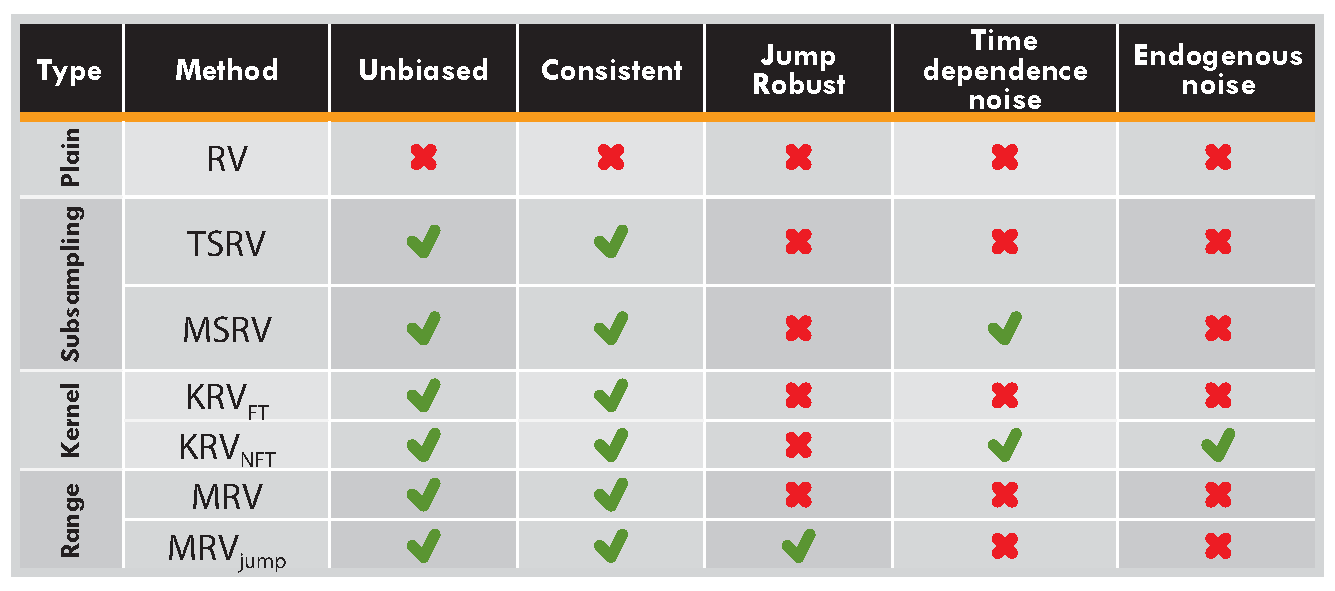
\includegraphics[scale=0.7]{img/Table}

\caption{Table Estimators}
\label{pic:TableEstimators}
\end{figure}


%------------------------------------------------------
\chapter{Price Noise Variance}
%------------------------------------------------------
\thispagestyle{plain}
%------------------------------------------------------
\section{RV Noise Variance}
%------------------------------------------------------
Assume that the observed (log) price is contaminated by market microstructure
noise $u$ (or measurement error), i.e.:
\begin{equation}
Y_{i/m} = X_{i/m} + u_{i/m}, \quad i = 1,2,\ldots, m
\end{equation}
where $X_{i/m}$ is the latent true, or so-called efficient, price that follows
the semimartingale. In this case, the observed intraday return is given
by:
\begin{equation}
r_i^{Y(m)} = r_i^{X(m)} + \epsilon_{i}^{(m)}, \quad i= 1,2,\ldots, m,
\end{equation}
i.e. by the efficient intraday return $r_i^{X(m)} = X_{i/m} - X_{(i-1)/m}$ and the intraday
noise increment $\epsilon_i^{(m)} = u_{i/m} - u_{(i-1)/m}$.\\

\noindent The noise variance $E\epsilon^2$ can be estiated consistently by normalized
realized variance over the whole interval $[0,1]$ for noisy data
~\cite[Zhang et al., 2005]{Zhang_Mykland_Ait-Sahalia}:
\begin{equation}
\label{Noise_Variance}
\hat{\omega}^2=\frac{1}{2n}\sum_{i=1}^{n} (Y_{t_i} - Y_{t_{i-1}})^2
\end{equation}
%------------------------------------------------------
\subsection{Properties}
\begin{itemize}
\item Convergence speed: $m^{1/2}$ ($m$ - number of observation)
\item Unbiased: no
\item Consistent: yes
\item Jump Robust: yes
\item Allows for time dependent noise: no
\end{itemize}

%------------------------------------------------------
\section{Autocovariance Noise Variance}
%------------------------------------------------------
The noise variance can be estimated as the negative of the first order autocovariance of observed returns ~\cite[Oomen, 2005]{Oomen}:
\begin{equation}
\label{AC_Variance}
\hat{\omega}^2=\max \left\{0, -\frac{1}{n-1}\sum_{i=1}^{n} (Y_{t_i} - Y_{t_{i-1}})(Y_{t_{i-1}} - Y_{t_{i-2}})\right\}
\end{equation}
%------------------------------------------------------
\subsection{Properties}
\begin{itemize}
\item Convergence speed: $m^{1/2}$ ($m$ - number of observation)
\item Unbiased: no
\item Consistent: yes
\item Jump Robust: yes
\item Allows for time dependent noise: no
\end{itemize}
  \subsection{Usage}
\begin{lstlisting}
noise_acnv(estimator)
\end{lstlisting}

%------------------------------------------------------
\chapter{Price Quarticity}

\section{Integrated Quarticity}
%------------------------------------------------------
The integrated quarticity is as described in ~\cite[Pigorsch et al.]{Pigorsch_Pigorsch_Popov}:
\begin{equation}
IQ = \int_{t-1}^t \sigma^4(s)ds.
\end{equation}
%-----------------------------------------------------
\section{Realized Quarticity}
%------------------------------------------------------
\subsection{Assumptions}
The microstructure noise.
\begin{enumerate}
\item The microstructure noise, $\epsilon_{t,i}$ , has zero mean and is an
independent and identically distributed random variable.
\item The noise is independent of the price process.
\item The variance of $\nu_{t,i} = \epsilon_{t,i} - \epsilon_{t,i-1}$ is
$O(1)$.
\end{enumerate}
%------------------------------------------------------
\subsection{Estimator}
The realized fourth-power variation or realized quarticity, defined as
~\cite[Corsi et al., 2005]{Corsi_Kretschmer_Mittnik_Pigorsch}:
\begin{equation}
\label{RQ}
RQ_t = \frac{M}{3} \sum_{j=1}^M r^4_{t,j} \stackrel{p}{\to} IQ
\end{equation}
where $M$ is sampling frequency.
  \subsection{Usage}
\begin{lstlisting}
quarticity_rq(estimator)
\end{lstlisting}
%------------------------------------------------------
\thispagestyle{plain}
%------------------------------------------------------
\section{Realized Quadpower Quarticity}
%------------------------------------------------------
\subsection{Assumptions}
The microstructure noise.
\begin{enumerate}
\item The microstructure noise, $\epsilon_{t,i}$ , has zero mean and is an
independent and identically distributed random variable.
\item The noise is independent of the price process.
\item The variance of $\nu_{t,i} = \epsilon_{t,i} - \epsilon_{t,i-1}$ is
$O(1)$.
\end{enumerate}
%------------------------------------------------------
\subsection{Estimator}
A more robust estimator then \ref{RQ} on p. \pageref{RQ}, especially
in the presence of jumps, is the realized quad-power quarticity ~\cite[Corsi et al., 2005]{Corsi_Kretschmer_Mittnik_Pigorsch}:
\begin{equation}
RQQ_t = M\frac{\pi^4}{4} \sum_{j=4}^M \mid r_{t,j} \mid \mid r_{t,j-1} \mid \mid
r_{t,j-2} \mid \mid r_{t,j-3} \mid \stackrel{p}{\to} IQ
\end{equation}
  \subsection{Usage}
\begin{lstlisting}
quarticity_rqq(estimator)
\end{lstlisting}
%------------------------------------------------------
%------------------------------------------------------
\thispagestyle{plain}
%------------------------------------------------------
\section{Modulated Realized Quarticity}
%------------------------------------------------------
\subsection{Assumptions}
The microstructure noise.
\begin{enumerate}
\item The microstructure noise, $\epsilon_{t,i}$ , has zero mean and is an
independent and identically distributed random variable.
\item The noise is independent of the price process.
\item The variance of $\nu_{t,i} = \epsilon_{t,i} - \epsilon_{t,i-1}$ is
$O(1)$.
\end{enumerate}
%------------------------------------------------------
\subsection{Estimator}
Modulated Realized Quarticity is written as ~\cite[Podolskij and Vetter, 2009]{Podolskij_Vetter}:
\begin{gather}
MRQ(Y)_n = \frac{(c_1 c_2/3)MBV(Y,4,0)_n - 2\nu_1\nu_2\hat{\omega}^2 MRV(Y)_n - \nu_2^2(\hat{\omega}^2)^2}{\nu_1^2} \stackrel{p}{\to} IQ
\end{gather}
where MBV is written as \ref{MBV} on p. \pageref{MBV},
\begin{gather}
\nu_1 = \frac{c_1(3c_2-4+(2-c_2)^3\bigvee 0)}{3(c_2-1)^2}
\end{gather}
\begin{gather}
\nu_2 = \frac{2((c_2-1)\bigwedge 1)}{c_1(c_2-1)^2}
\end{gather}
We can choose the constants $c_1$ and $c_2$ from specific process:
\begin{equation}
c_1 = 0.25, \quad
c_2 = 2.
\end{equation}
%------------------------------------------------------
\subsection{Properties}
\begin{itemize}
\item Convergence speed: $m^{1/4}$ ($m$ - number of observation)
\item Unbiased: yes
\item Consistent: yes
\item Jump Robust: no
\item Allows for time dependence noise: no
\item Allows for for endogenous noise: no
\end{itemize}
  \subsection{Usage}
\begin{lstlisting}
quarticity_mrq(estimator)
\end{lstlisting}
%------------------------------------------------------

\begin{thebibliography}{100}
\bibitem{Pigorsch_Pigorsch_Popov}U. Pigorsch, C. Pigorsch, I. Popov, "Volatility estimation based on high-frequency data", In: Duan, JC, Gentle, JE and Hardle E, Handbook of Computational Finance, New York: Springer, 2010
\bibitem{Zu_Boswijk}Y. Zu and Peter Boswijk, "Estimating spot volatility with high-frequency financial data", Journal of Econometrics, 181(2), pp. 117-135, 2014
\bibitem{Zhang_Mykland_Ait-Sahalia}L. Zhang, P. A. Mykland, and Y. Ait-Sahalia, "A tale of two time scales: Determining integrated volatility with noisy high-frequency data", Journal of the American Statistical Association, vol. 100, No. 472, pp. 1394-1411, 2005.
\bibitem{Podolskij_Vetter}M. Podolskij and M. Vetter, "Estimation of volatility functionals in the simultaneous presence of microstructure noise and jumps", Bernoulli, vol. 15, No. 3, pp. 634-658, 2009.
\bibitem{BarndorffNielsen_Hansen_Lunde_Shephard}O.E.Barndorff-Nielsen, P.Reinhard Hansen, A.Lunde, and N.Shephard, "Designing realised kernels to measure the ex-post variation of equity prices in the presence of noise", Economics Series Working Papers 264, University of Oxford, Department of Economics, 2006.
\bibitem{Oomen}R. C. Oomen, "Comment on realized variance and market microstructure noise by Peter R. Hansen and Asger Lunde," pp. 1-15, 2005.
\bibitem{Corsi_Kretschmer_Mittnik_Pigorsch} Corsi, F., U. Kretschmer, S. Mittnik and C. Pigorsch, "The Volatility of Realized Volatility", Econometric Reviews, pp. 46-78, 2008
\end{thebibliography} 
 
\end{document}


